\documentclass[11pt]{article}
\usepackage{amsmath, amssymb, amsthm}
\usepackage{geometry}
\usepackage{setspace}
\usepackage{minted}
\usepackage{graphicx}
\usepackage{url}

\geometry{margin=1in}
\setlength{\parindent}{0pt}

\title{Homework 2}
\author{Andrew Wang}
\date{27 January 2026}

\begin{document}
\maketitle

\section{Problem 1}

\section*{Problem 1 (10 pts)}

Prove that the Continuous Ranked Probability Score (CRPS) is the univariate case of the energy score. That is, for a cumulative distribution function $F$, we have

\[
\int_{-\infty}^{+\infty} \left[ F(x) - \mathbf{1}\{ y \le x \} \right]^2 \, dx
=
\mathbb{E}_F \left| Y - y \right|
-
\frac{1}{2} \mathbb{E}_F \left| Y - Y' \right|,
\]

where $Y, Y'$ are two independent draws from $F$.

\medskip

\noindent\textbf{Hint:} Use the identity
\[
|x - y|
=
\int_{-\infty}^{+\infty}
\left[
\mathbf{1}\{ x \le u < y \}
+
\mathbf{1}\{ y \le u < x \}
\right]
\, du.
\]

\hrulefill

\textbf{Proof}

We begin from the right-hand side, making use of the identity as follows:
\begin{align}
    \mathbb{E}_F \left| Y - y \right|
    -
    \frac{1}{2} \mathbb{E}_F \left| Y - Y' \right| &=
    \underbrace{\mathbb{E}_F \int_{-\infty}^{\infty}\mathbf{1}[Y \leq x < y] + \mathbf{1}[y \leq x < Y] \; dx}_{\mathbf{(1)}} \nonumber \\
    &-
    \frac{1}{2} \underbrace{\mathbb{E}_F \int_{-\infty}^{\infty}\mathbf{1}[Y \leq x < Y'] + \mathbf{1}[Y' \leq x < Y] \; dx}_{\mathbf{(2)}}. \label{p1}
\end{align}

For $\mathbf{(1)}$, we can show:
\begin{align}
    \mathbf{(1)} &= \int_{-\infty}^{\infty} \mathbb{P}(Y \leq x < y) + \mathbb{P}(y \leq x < Y) \; dx \nonumber \\
    &= \int_{-\infty}^{\infty} F(x) \mathbf{1}(x \leq y) + \big( 1 - F(x) \big) \mathbf{1}(y \leq x) \; dx \nonumber \\
    &= \int_{-\infty}^{y} F(x) \; dx + \int_{y}^{\infty} 1 - F(x) \; dx. \label{p1.1}
\end{align}

For $\mathbf{(2)}$, we can show:
\begin{align}
    \mathbf{(2)} &= \int_{-\infty}^{\infty} \mathbb{P} (Y \leq x < Y') + \mathbb{P} (Y' \leq x < Y) \; dx \nonumber \\
    &= \int_{-\infty}^{\infty} \mathbb{P} (Y \leq x ) \mathbb{P} (x < Y') + \mathbb{P} (Y' \leq x) \mathbb{P} (x < Y) \; dx \label{p1pt2}\\
    &=\int_{-\infty}^{\infty} 2F(x) \big( 1 - F(x) \big) \; dx, \label{p1.2}
\end{align}
where expression \ref{p1pt2} is true since $Y \perp Y'$. Now we can make use of expressions \ref{p1.1} and \ref{p1.2} to demonstrate that expression \ref{p1} is:
\begin{align*}
    \mathbb{E}_F \left| Y - y \right|
    -
    \frac{1}{2} \mathbb{E}_F \left| Y - Y' \right| &=
    \int_{-\infty}^{y} F(x) \; dx + \int_{y}^{\infty} 1 - F(x) \; dx - \int_{-\infty}^{\infty} F(x) \big( 1 - F(x) \big) \; dx \\
    &= \int_{-\infty}^{y} F(x) \; dx + \int_{y}^{\infty} 1 - F(x) \; dx - \int_{-\infty}^{y} F(x) \big( 1 - F(x) \big) \; dx - \int_{y}^{\infty} F(x) \big( 1 - F(x) \big) \; dx \\
    &= \int_{-\infty}^{y} F(x)^2 \; dx + \int_{y}^{\infty} \big( 1 - F(x) \big) ^2 \; dx \\
    &= \int_{-\infty}^{+\infty} \left[ F(x) - \mathbf{1}\{ y \le x \} \right]^2 \; dx,
\end{align*}
which proves the given claim.

\section{Problem 2}

I used a normalizing flow with the \texttt{normflow} library, though the coupling flow taught in lecture was not applicable as we are predicting an unconditional density. I used a rational quadratic spline.
\begin{itemize}
    \item Energy Distance: 0.035
    \item Wasserstein Distance: 0.071
\end{itemize}

\begin{figure}[htbp!]
    \centering
    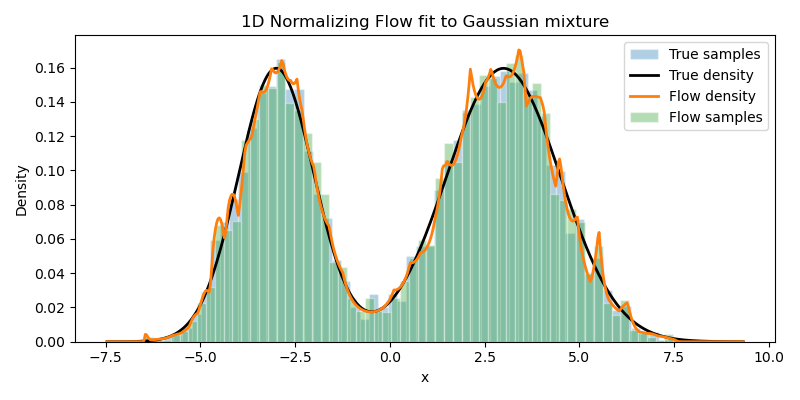
\includegraphics[width=0.7\linewidth]{HW2Q2_1.png}
    \caption{}
    \label{fig:normflow}
\end{figure}

I then used engression, with the following results:
\begin{itemize}
    \item Energy Distance: 0.161
    \item Wasserstein Distance: 0.369
\end{itemize}

\begin{figure}[htbp!]
    \centering
    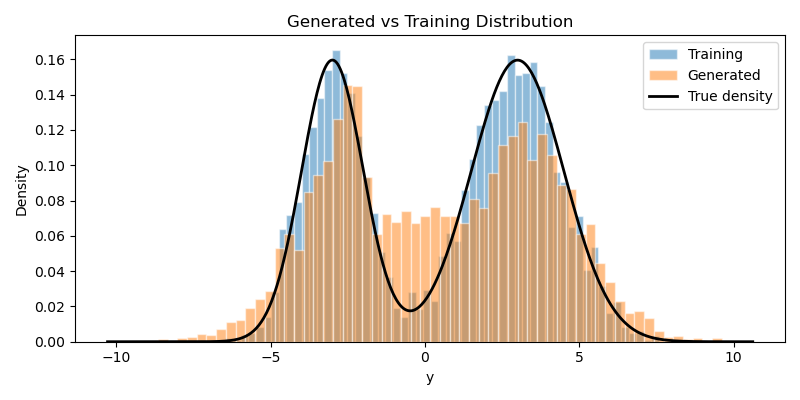
\includegraphics[width=0.7\linewidth]{HW2Q2_2.png}
    \caption{}
    \label{fig:engress}
\end{figure}

The full code can be found attached.

\end{document}
